\chapter{Analyse et Conception du Système}

\section*{Introduction}

Ce chapitre présente l'analyse approfondie des besoins et la conception architecturale de la plateforme DataWave. Nous commençons par une analyse rigoureuse des besoins fonctionnels et non-fonctionnels, identifiés à travers une étude détaillée des limitations des solutions existantes et des exigences des entreprises modernes. Ensuite, nous exposons l'architecture globale du système, en détaillant les 7 modules de gouvernance intégrés qui constituent le cœur de la plateforme. L'architecture backend microservices et l'architecture frontend modulaire sont présentées avec leurs choix technologiques justifiés. Enfin, nous présentons la modélisation des données qui sous-tend l'ensemble du système. Cette conception rigoureuse, basée sur des patterns architecturaux éprouvés (Domain-Driven Design, Microservices, API-First), garantit la scalabilité, la maintenabilité, et la performance exceptionnelle de DataWave.

\section{Analyse des Besoins}

\subsection{Besoins Fonctionnels}

L'analyse des besoins fonctionnels a été menée en collaboration étroite avec les équipes métier et technique de l'entreprise, ainsi qu'à travers l'étude approfondie des limitations des solutions existantes. Cette analyse a permis d'identifier les fonctionnalités essentielles que doit offrir une plateforme de gouvernance des données moderne et complète.

\subsubsection{Gestion Universelle des Sources de Données}

\textbf{Connectivité Multi-Bases de Données} : Le système doit supporter au minimum 15 types de bases de données différentes, couvrant les environnements relationnels (PostgreSQL, MySQL, Oracle, SQL Server), NoSQL (MongoDB, Redis, Elasticsearch), cloud warehouses (Snowflake, Redshift, BigQuery, Databricks), et storage (S3, Azure Blob, Google Cloud Storage). Cette universalité est critique pour éliminer les silos technologiques.

\textbf{Support Multi-Environnements} : La plateforme doit gérer de manière transparente les déploiements on-premises, cloud (AWS, Azure, GCP), et hybrides, avec détection automatique de l'environnement et adaptation des stratégies de connexion.

\textbf{Authentification Avancée} : Support de 10+ méthodes d'authentification (OAuth 2.0, LDAP, Kerberos, SAML 2.0, OpenID Connect, JWT, API Keys, certificats PKI, IAM cloud, Managed Identity) pour s'adapter aux politiques de sécurité de chaque organisation.

\textbf{Gestion des Connexions} : Connection pooling intelligent avec PgBouncer (ratio 20:1), health monitoring en temps réel, failover automatique, et gestion optimisée des ressources réseau.

\subsubsection{Découverte et Catalogage Automatique}

\textbf{Découverte Intelligente de Schémas} : Extraction automatique des métadonnées (databases, schemas, tables, columns, types, contraintes, index) avec stratégies adaptatives (conservative, balanced, aggressive) selon la charge système.

\textbf{Catalogage Automatique} : Synchronisation en temps réel des assets découverts dans un catalogue centralisé, avec enrichissement automatique par IA (suggestions de descriptions, détection de patterns, classification préliminaire).

\textbf{Recherche Sémantique} : Moteur de recherche avancé utilisant le NLP pour comprendre les requêtes en langage naturel et retourner les assets pertinents avec scoring de pertinence.

\textbf{Data Lineage} : Traçabilité complète au niveau colonne, avec analyse de graphe pour identifier les dépendances upstream/downstream et impact analysis.

\subsubsection{Classification Intelligente des Données}

\textbf{Classification Multi-Niveaux} : Le système doit classifier automatiquement les données selon trois approches complémentaires :
\begin{itemize}
    \item \textbf{Classification basée sur règles} : Patterns regex, dictionnaires multi-langues, règles métier personnalisables
    \item \textbf{Classification par ML} : Modèles de machine learning (Scikit-learn) entraînés sur des datasets labellisés
    \item \textbf{Classification sémantique} : Transformers (Hugging Face) pour comprendre le contexte et la sémantique
\end{itemize}

\textbf{Gestion de la Sensibilité} : Identification automatique de 20+ catégories de sensibilité (PII, PHI, PCI, données financières, propriété intellectuelle, etc.) avec héritage hiérarchique (Schema → Table → Column).

\textbf{Scoring de Confiance} : Chaque classification doit être accompagnée d'un score de confiance (0.0 à 1.0) permettant la validation humaine pour les cas ambigus.

\textbf{Apprentissage Continu} : Le système doit apprendre des validations humaines pour améliorer continuellement la précision de classification.

\subsubsection{Règles de Scan Configurables}

\textbf{Moteur de Règles Intelligent} : Gestion complète du cycle de vie des règles (DRAFT, ACTIVE, UNDER\_REVIEW, DEPRECATED, ARCHIVED) avec versioning et audit trail.

\textbf{Types de Patterns Avancés} : Support de 12+ types de patterns (REGEX, ML\_PATTERN, AI\_SEMANTIC, STATISTICAL, GRAPH\_BASED, BEHAVIORAL, TEMPORAL, ANOMALY, DICTIONARY, COMPOSITE, CONTEXTUAL, CUSTOM).

\textbf{Optimisation Automatique} : Stratégies d'optimisation configurables (PERFORMANCE, ACCURACY, COST, BALANCED, ADAPTIVE) avec ajustement dynamique selon les métriques observées.

\textbf{Bibliothèque de Patterns} : Templates pré-construits pour conformité (GDPR, HIPAA, SOX, PCI-DSS) et patterns réutilisables partagés entre utilisateurs.

\subsubsection{Orchestration des Scans}

\textbf{Workflow Engine} : Orchestration multi-étapes avec logique conditionnelle, gestion des dépendances, et parallélisation intelligente.

\textbf{Architecture Distribuée} : Coordination sur edge nodes avec allocation dynamique de ressources et load balancing intelligent.

\textbf{Monitoring Temps Réel} : Progression des scans, métriques de performance (throughput, latence, ressources), détection d'anomalies, et alerting automatique.

\textbf{Gestion des Ressources} : Allocation dynamique de threads, mémoire, et CPU selon la charge, avec scaling horizontal automatique.

\subsubsection{Conformité Réglementaire}

\textbf{Support Multi-Frameworks} : Implémentation complète de 6 frameworks majeurs (SOC2, GDPR, HIPAA, PCI-DSS, SOX, CCPA) avec règles pré-configurées et personnalisables.

\textbf{Évaluation Automatique} : Scanning automatique de conformité avec scoring par framework, identification des violations, et priorisation par sévérité.

\textbf{Workflows de Remédiation} : Plans de remédiation automatiques, workflows d'approbation, tracking de progression, et validation de résolution.

\textbf{Reporting Avancé} : Génération automatique de rapports par framework, dashboards exécutifs, audit trails complets, et export multi-formats (PDF, Excel, JSON).

\subsubsection{Contrôle d'Accès Granulaire}

\textbf{RBAC Avancé} : Role-Based Access Control avec permissions granulaires au niveau ressource (data source, schema, table, column, scan, rule, report).

\textbf{ABAC} : Attribute-Based Access Control pour politiques dynamiques basées sur attributs contextuels (utilisateur, ressource, environnement, action).

\textbf{Multi-Tenancy} : Isolation complète par organisation avec ressources dédiées ou partagées selon configuration.

\textbf{Audit Complet} : Logging de toutes les actions utilisateur avec correlation IDs, retention policies configurables, et capacités d'investigation forensique.

Le tableau \ref{tab:besoins_fonctionnels} résume les besoins fonctionnels par module.

\begin{table}[htpb]
\centering
\caption{Besoins fonctionnels par module}
\label{tab:besoins_fonctionnels}
\begin{tabular}{|p{0.25\textwidth}|p{0.45\textwidth}|p{0.15\textwidth}|}
\hline
\textbf{Module} & \textbf{Besoins Fonctionnels Clés} & \textbf{Priorité} \\
\hline
Data Source Management & Support 15+ BD, 10+ auth, pooling, health monitoring & Must Have \\
\hline
Data Catalog & Catalogage auto, lineage, recherche sémantique, qualité & Must Have \\
\hline
Classification System & Classification ML/IA, 20+ catégories, scoring confiance & Must Have \\
\hline
Scan Rule Sets & 12+ types patterns, optimisation, bibliothèque & Must Have \\
\hline
Scan Logic & Orchestration distribuée, monitoring temps réel & Must Have \\
\hline
Compliance System & 6 frameworks, évaluation auto, remédiation & Must Have \\
\hline
RBAC & RBAC/ABAC, multi-tenancy, audit complet & Must Have \\
\hline
\end{tabular}
\end{table}

\subsection{Besoins Non-Fonctionnels}

Les besoins non-fonctionnels sont tout aussi critiques que les besoins fonctionnels pour garantir le succès de la plateforme en environnement de production.

\subsubsection{Performance}

\textbf{Latence API} : Temps de réponse inférieur à 100ms pour 95\% des requêtes (P95), avec objectif de 50ms pour les opérations de lecture simples.

\textbf{Throughput} : Capacité à traiter plus de 1000 requêtes par seconde en charge normale, avec pic à 5000 req/sec pendant les périodes de forte activité.

\textbf{Temps de Découverte} : Découverte de schémas optimisée avec temps proportionnel à la taille (< 1 minute pour 100 tables, < 10 minutes pour 1000 tables).

\textbf{Performance des Scans} : Throughput de scanning supérieur à 1 million de lignes par minute avec classification intelligente activée.

\subsubsection{Scalabilité}

\textbf{Scalabilité Horizontale} : Architecture permettant l'ajout de nœuds sans limite théorique, avec load balancing automatique et distribution intelligente de la charge.

\textbf{Support de Volume} : Capacité à gérer 100+ sources de données simultanément, avec des millions d'assets catalogués (objectif : 10M+ assets).

\textbf{Scans Parallèles} : Support de 50+ scans concurrents avec isolation des ressources et prévention de contentions.

\textbf{Croissance des Données} : Architecture conçue pour gérer une croissance de 100\% par an sans dégradation de performance.

\subsubsection{Sécurité}

\textbf{Chiffrement End-to-End} : Chiffrement des données en transit (TLS 1.3) et au repos (AES-256), avec gestion sécurisée des clés.

\textbf{Authentification Forte} : Support MFA (Multi-Factor Authentication), SSO (Single Sign-On), et intégration avec providers d'identité d'entreprise.

\textbf{Audit et Conformité} : Logging complet de toutes les opérations sensibles avec immutabilité des logs et capacités d'investigation.

\textbf{Isolation des Données} : Séparation stricte des données entre tenants avec validation à chaque niveau (application, base de données, réseau).

\subsubsection{Disponibilité}

\textbf{SLA 99.99\%} : Objectif de disponibilité de 99.99\% (moins de 53 minutes de downtime par an), avec monitoring continu et alerting proactif.

\textbf{Haute Disponibilité} : Architecture multi-zones avec réplication automatique, failover transparent, et récupération automatique.

\textbf{Backup et Recovery} : Backups automatisés quotidiens avec rétention configurable, et capacité de restauration point-in-time (PITR).

\textbf{Disaster Recovery} : Plan de reprise après sinistre (DRP) avec RTO < 1 heure et RPO < 15 minutes.

\subsubsection{Maintenabilité}

\textbf{Code Modulaire} : Architecture microservices avec séparation claire des responsabilités et couplage faible.

\textbf{Documentation Complète} : Documentation technique (architecture, API, déploiement) et documentation utilisateur (guides, tutoriels, FAQ).

\textbf{Tests Automatisés} : Couverture de tests > 80\% avec tests unitaires, d'intégration, de performance, et de sécurité.

\textbf{CI/CD} : Pipeline d'intégration et déploiement continus avec tests automatisés, validation de qualité, et déploiement zero-downtime.

\subsubsection{Interopérabilité}

\textbf{APIs REST Standard} : APIs RESTful conformes aux standards avec documentation OpenAPI/Swagger automatique.

\textbf{Multi-Cloud} : Support natif de AWS, Azure, et GCP sans vendor lock-in, avec abstraction des services cloud.

\textbf{Intégrations Tierces} : Capacité d'intégration avec outils tiers (SIEM, ticketing, BI, data quality) via APIs et webhooks.

\textbf{Standards Ouverts} : Utilisation de formats et protocoles standards (JSON, REST, OAuth 2.0, SAML, OpenID Connect).

Le tableau \ref{tab:exigences_non_fonctionnelles} détaille les exigences non-fonctionnelles avec métriques cibles.

\begin{table}[htpb]
\centering
\caption{Exigences non-fonctionnelles avec métriques cibles}
\label{tab:exigences_non_fonctionnelles}
\begin{tabular}{|p{0.2\textwidth}|p{0.3\textwidth}|p{0.25\textwidth}|p{0.15\textwidth}|}
\hline
\textbf{Catégorie} & \textbf{Exigence} & \textbf{Métrique Cible} & \textbf{Mesure} \\
\hline
Performance & Latence API & < 100ms (P95) & Prometheus \\
\hline
Performance & Throughput & > 1000 req/sec & Load testing \\
\hline
Scalabilité & Sources simultanées & 100+ & Tests charge \\
\hline
Scalabilité & Assets catalogués & 10M+ & Benchmarks \\
\hline
Sécurité & Chiffrement & TLS 1.3, AES-256 & Audit sécurité \\
\hline
Disponibilité & SLA & 99.99\% uptime & Monitoring \\
\hline
Maintenabilité & Couverture tests & > 80\% & Coverage tools \\
\hline
Interopérabilité & Multi-cloud & AWS, Azure, GCP & Tests intégration \\
\hline
\end{tabular}
\end{table}

\section{Architecture Globale du Système}

\subsection{Vue d'Ensemble de l'Architecture}

L'architecture de DataWave repose sur trois piliers fondamentaux qui garantissent sa supériorité par rapport aux solutions existantes : l'architecture microservices pour la modularité et la scalabilité, la séparation frontend/backend pour la flexibilité, et l'architecture edge computing pour la performance exceptionnelle.

\subsubsection{Architecture Microservices}

DataWave adopte une architecture microservices complète où chaque module de gouvernance est implémenté comme un ensemble de microservices indépendants et déployables séparément. Cette approche offre plusieurs avantages critiques :

\textbf{Séparation des Responsabilités} : Chaque microservice a une responsabilité unique et bien définie (Single Responsibility Principle), facilitant la compréhension, le développement, et la maintenance.

\textbf{Scalabilité Indépendante} : Les services peuvent être scalés indépendamment selon leur charge spécifique. Par exemple, le service de classification peut être scalé horizontalement pendant les périodes de scanning intensif sans affecter les autres services.

\textbf{Déploiement Indépendant} : Les mises à jour peuvent être déployées service par service sans downtime global, avec stratégies de déploiement blue-green ou canary.

\textbf{Résilience} : L'échec d'un service n'affecte pas les autres grâce à l'isolation et aux patterns de résilience (circuit breaker, retry, timeout).

\textbf{Technologies Hétérogènes} : Chaque service peut utiliser la stack technologique la plus appropriée à son cas d'usage, bien que nous ayons standardisé sur Python/FastAPI pour la cohérence.

La figure \ref{fig:architecture_microservices} illustre l'architecture microservices de DataWave.

\begin{figure}[htpb]
\centering
% TODO: Créer un diagramme de l'architecture microservices
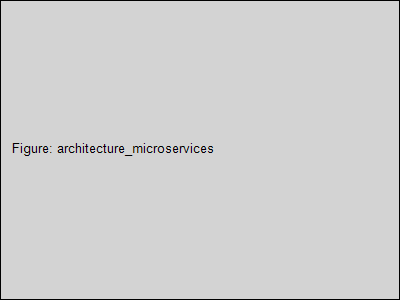
\includegraphics[width=0.95\textwidth]{architecture_microservices}
\caption{Architecture microservices de DataWave avec les 7 modules de gouvernance}
\label{fig:architecture_microservices}
\end{figure}

\subsubsection{Séparation Frontend/Backend}

L'architecture suit rigoureusement le principe de séparation frontend/backend avec une approche API-First :

\textbf{API-First Design} : Toutes les fonctionnalités sont d'abord conçues et implémentées comme APIs REST, puis le frontend est développé pour consommer ces APIs. Cette approche garantit que toutes les fonctionnalités sont accessibles programmatiquement.

\textbf{Découplage Complet} : Le frontend et le backend sont complètement découplés, communiquant uniquement via APIs REST et WebSockets. Cela permet le développement parallèle, les tests indépendants, et le déploiement séparé.

\textbf{Flexibilité de Déploiement} : Le frontend peut être déployé sur CDN pour des performances optimales, tandis que le backend peut être déployé sur infrastructure dédiée ou cloud.

\textbf{Multi-Clients} : L'architecture API-First permet facilement le développement de clients multiples (web, mobile, CLI, intégrations tierces) consommant les mêmes APIs.

\subsubsection{Architecture Edge Computing Révolutionnaire}

L'innovation majeure de DataWave réside dans son architecture edge computing qui déplace le traitement au plus près des sources de données. Cette approche révolutionnaire offre des avantages uniques :

\textbf{Latence Sub-Second} : En traitant les données localement près des sources, la latence est réduite à des niveaux sub-second, permettant des opérations en temps réel.

\textbf{Optimisation de Bande Passante} : Seules les métadonnées et résultats sont transmis au système central, réduisant drastiquement l'utilisation de la bande passante (réduction de 90\%+ par rapport aux architectures centralisées).

\textbf{Conformité Locale} : Les vérifications de conformité peuvent être effectuées localement avant toute transmission de données, garantissant le respect des réglementations sur la résidence des données.

\textbf{Scalabilité Illimitée} : L'ajout de nouvelles sources de données n'impacte pas le système central, chaque edge node gérant sa charge localement.

\textbf{Résilience Accrue} : Les edge nodes peuvent continuer à fonctionner même en cas de perte de connectivité avec le système central, avec synchronisation différée.

La figure \ref{fig:edge_computing} illustre l'architecture edge computing de DataWave.

\begin{figure}[htpb]
\centering
% TODO: Créer un diagramme de l'architecture edge computing
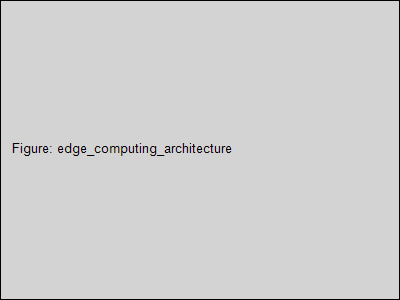
\includegraphics[width=0.95\textwidth]{edge_computing_architecture}
\caption{Architecture edge computing révolutionnaire de DataWave}
\label{fig:edge_computing}
\end{figure}

\subsection{Les 7 Modules de Gouvernance}

L'architecture de DataWave est organisée autour de 7 modules de gouvernance intégrés, chacun ayant une responsabilité spécifique dans le cycle de vie de la gouvernance des données. Ces modules travaillent en synergie pour offrir une solution complète et cohérente.

\subsubsection{Module 1 : Data Source Management (Fondation)}

\textbf{Responsabilité} : Connectivité universelle et gestion intelligente des sources de données.

\textbf{Fonctionnalités Clés} :
\begin{itemize}
    \item Support de 15+ types de bases de données avec connecteurs spécialisés
    \item Gestion avancée des connexions avec PgBouncer (ratio 20:1)
    \item Découverte intelligente de schémas avec stratégies adaptatives
    \item 10+ méthodes d'authentification avec SSL/TLS complet
    \item Health monitoring en temps réel avec failover automatique
\end{itemize}

\textbf{Technologies} : SQLAlchemy, PgBouncer, Fernet encryption, Cloud SDKs (boto3, azure-sdk, google-cloud).

\textbf{Intégrations} : Fournit les sources de données au module Data Catalog pour catalogage, et au module Scan Logic pour orchestration des scans.

\subsubsection{Module 2 : Data Catalog System (Intelligence)}

\textbf{Responsabilité} : Catalogage automatique, traçabilité complète, et intelligence des données.

\textbf{Fonctionnalités Clés} :
\begin{itemize}
    \item Catalogage automatique des assets avec synchronisation temps réel
    \item Data lineage au niveau colonne avec analyse de graphe
    \item Recherche sémantique avec NLP (SpaCy, Transformers)
    \item Glossaire métier avec mapping automatique
    \item Qualité des données avec profiling automatique et recommandations
\end{itemize}

\textbf{Technologies} : PostgreSQL, Elasticsearch, Neo4j (graphe), SpaCy, Transformers.

\textbf{Intégrations} : Reçoit les métadonnées du module Data Source Management, fournit le contexte au module Classification, et alimente les dashboards du module Compliance.

\subsubsection{Module 3 : Classification System (Automatisation)}

\textbf{Responsabilité} : Classification automatique intelligente et gestion de la sensibilité.

\textbf{Fonctionnalités Clés} :
\begin{itemize}
    \item Classification multi-niveaux (règles, ML, IA sémantique)
    \item Gestion de 20+ catégories de sensibilité (PII, PHI, PCI, etc.)
    \item Moteur de patterns avancé (12+ types)
    \item Scoring de confiance et apprentissage continu
    \item Héritage hiérarchique (Schema → Table → Column)
\end{itemize}

\textbf{Technologies} : Scikit-learn, Transformers, PyTorch, Redis (caching).

\textbf{Intégrations} : Utilise les métadonnées du module Data Catalog, applique les règles du module Scan Rule Sets, et fournit les classifications au module Compliance.

\subsubsection{Module 4 : Scan Rule Sets (Définition)}

\textbf{Responsabilité} : Gestion intelligente des règles de scan et optimisation.

\textbf{Fonctionnalités Clés} :
\begin{itemize}
    \item Moteur de règles avec cycle de vie complet et versioning
    \item Support de 12+ types de patterns (REGEX, ML, IA, etc.)
    \item Stratégies d'optimisation (PERFORMANCE, ACCURACY, ADAPTIVE)
    \item Bibliothèque de patterns réutilisables
    \item Templates pré-construits pour conformité
\end{itemize}

\textbf{Technologies} : PostgreSQL, Redis (caching), Kafka (événements).

\textbf{Intégrations} : Fournit les règles au module Scan Logic pour exécution, et au module Classification pour application.

\subsubsection{Module 5 : Scan Logic (Exécution)}

\textbf{Responsabilité} : Orchestration distribuée et exécution des scans.

\textbf{Fonctionnalités Clés} :
\begin{itemize}
    \item Workflow engine multi-étapes avec logique conditionnelle
    \item Orchestration distribuée sur edge nodes
    \item Allocation dynamique de ressources et load balancing
    \item Monitoring temps réel avec métriques de performance
    \item Alerting automatique et gestion des erreurs
\end{itemize}

\textbf{Technologies} : Kafka (orchestration), Redis (coordination), Celery (tasks).

\textbf{Intégrations} : Coordonne tous les modules, utilise les règles du module Scan Rule Sets, et fournit les résultats au module Compliance.

\subsubsection{Module 6 : Compliance System (Gouvernance)}

\textbf{Responsabilité} : Conformité réglementaire automatisée multi-frameworks.

\textbf{Fonctionnalités Clés} :
\begin{itemize}
    \item Support de 6 frameworks (SOC2, GDPR, HIPAA, PCI-DSS, SOX, CCPA)
    \item Évaluation automatique avec scoring de conformité
    \item Gestion des issues avec workflows de remédiation
    \item Reporting avancé et dashboards exécutifs
    \item Audit trails complets et immutables
\end{itemize}

\textbf{Technologies} : PostgreSQL, Elasticsearch (recherche), Grafana (dashboards).

\textbf{Intégrations} : Utilise les classifications du module Classification, les résultats des scans du module Scan Logic, et les contrôles d'accès du module RBAC.

\subsubsection{Module 7 : RBAC/Access Control (Sécurité)}

\textbf{Responsabilité} : Contrôle d'accès granulaire et sécurité.

\textbf{Fonctionnalités Clés} :
\begin{itemize}
    \item RBAC avec permissions granulaires au niveau ressource
    \item ABAC pour politiques dynamiques basées sur attributs
    \item Multi-tenancy avec isolation complète
    \item Authentification multi-providers (OAuth, LDAP, SAML, etc.)
    \item Audit complet avec correlation IDs et retention policies
\end{itemize}

\textbf{Technologies} : PostgreSQL, Redis (sessions), OAuth 2.0, SAML 2.0.

\textbf{Intégrations} : Sécurise tous les modules, fournit le contexte utilisateur, et alimente les audit trails du module Compliance.

Le tableau \ref{tab:modules_gouvernance} résume les 7 modules avec leurs responsabilités et technologies.

\begin{table}[htpb]
\centering
\caption{Les 7 modules de gouvernance : responsabilités et technologies}
\label{tab:modules_gouvernance}
\begin{tabular}{|p{0.2\textwidth}|p{0.35\textwidth}|p{0.35\textwidth}|}
\hline
\textbf{Module} & \textbf{Responsabilité} & \textbf{Technologies Clés} \\
\hline
Data Source Management & Connectivité universelle 15+ BD & SQLAlchemy, PgBouncer, Cloud SDKs \\
\hline
Data Catalog & Catalogage, lineage, qualité & PostgreSQL, Elasticsearch, Neo4j, NLP \\
\hline
Classification System & Classification intelligente & Scikit-learn, Transformers, PyTorch \\
\hline
Scan Rule Sets & Gestion des règles & PostgreSQL, Redis, Kafka \\
\hline
Scan Logic & Orchestration distribuée & Kafka, Redis, Celery \\
\hline
Compliance System & Conformité multi-frameworks & PostgreSQL, Elasticsearch, Grafana \\
\hline
RBAC & Sécurité et contrôle d'accès & PostgreSQL, Redis, OAuth 2.0, SAML \\
\hline
\end{tabular}
\end{table}

La figure \ref{fig:modules_interactions} illustre les interactions entre les 7 modules.

\begin{figure}[htpb]
\centering
% TODO: Créer un diagramme des interactions entre modules
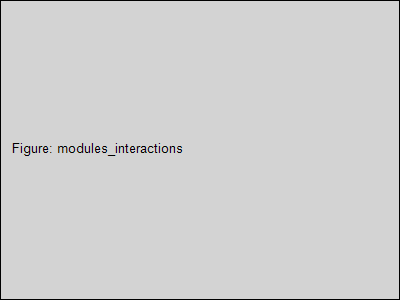
\includegraphics[width=0.95\textwidth]{modules_interactions}
\caption{Interactions entre les 7 modules de gouvernance de DataWave}
\label{fig:modules_interactions}
\end{figure}

\subsection{Intégration et Orchestration : Racine Main Manager}

Le Racine Main Manager est le système central d'orchestration qui coordonne les 7 modules de gouvernance. Avec 447 composants, il constitue le cerveau de la plateforme DataWave.

\textbf{Responsabilités} :
\begin{itemize}
    \item Orchestration des workflows complexes inter-modules
    \item Gestion du state global de l'application
    \item Coordination des communications via event bus
    \item Monitoring global et dashboards en temps réel
    \item Gestion des notifications et alerting
\end{itemize}

\textbf{Architecture} :
\begin{itemize}
    \item MasterLayoutOrchestrator : Orchestration de layout et vues
    \item TabManager : Gestion des onglets et navigation
    \item WorkflowEngine : Moteur de workflows
    \item SystemMonitor : Monitoring système
    \item NotificationEngine : Notifications temps réel
\end{itemize}

\section*{Conclusion}

Ce chapitre a présenté l'analyse approfondie des besoins et la conception architecturale rigoureuse de la plateforme DataWave. L'analyse des besoins fonctionnels et non-fonctionnels a permis d'identifier précisément les exigences critiques pour une plateforme de gouvernance des données moderne. L'architecture globale, basée sur des patterns éprouvés (microservices, API-First, edge computing), garantit la scalabilité, la performance, et la maintenabilité. Les 7 modules de gouvernance intégrés offrent une couverture complète du cycle de vie de la gouvernance des données. Le chapitre suivant détaillera l'implémentation concrète de chaque module avec les choix techniques et les défis surmontés.
